\newpage
\section{Backend}
\subsection{Overview}
The backend of the meta learning system is arguably one of the most important components, as it is responsible for storing and 
organising data. Additionally, this component will be appropriately implemented to optimise the LMS runtimes.

The backend component will have no user interface and will only include the database, data, endpoints and documentation. In addition, 
the backend component will list all the endpoints via documentation. This component will only be accessible to developers and admins through 
a combination of both backend files and a command terminal.

Overall, the successful implementation of the backend component of the LMS will constitute the foundation of the LMS and 
ensure effective runtimes for the entire LMS system.

\subsection{Design}
There will be many database schemas which will be implemented in the backend. These schemas will be dependant on the requirements for each 
feature. For example, the schema for the lectures and tutorials feature will include relations between lectures and lecturers.  

Moreover, an example of a table structure for the lectures and tutorials will include: the lecture id, the lecture title, the 
lecture associated files, the lecturers in charge and the enrolled students in the lecture. 

\begin{figure}[h!]
    \centering
    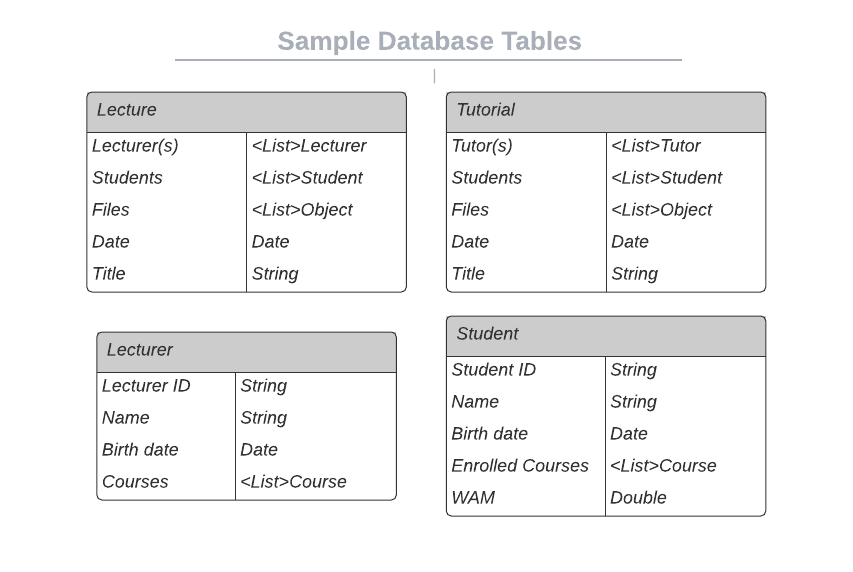
\includegraphics[scale=0.6]{backend_sample_tables}
    \caption{Sample Database Tables}
\end{figure}

The calls that can be made to the backend will include data retrieval, updates, creation and deleting. An example of such a 
creation call is creating a lecture entry. Moreover, the calls samples will be further updated in the future to include a variety 
of calls for different schemas. For instance, a GET request for students enrolled in a course.

\begin{figure}[h!]
  \centering
  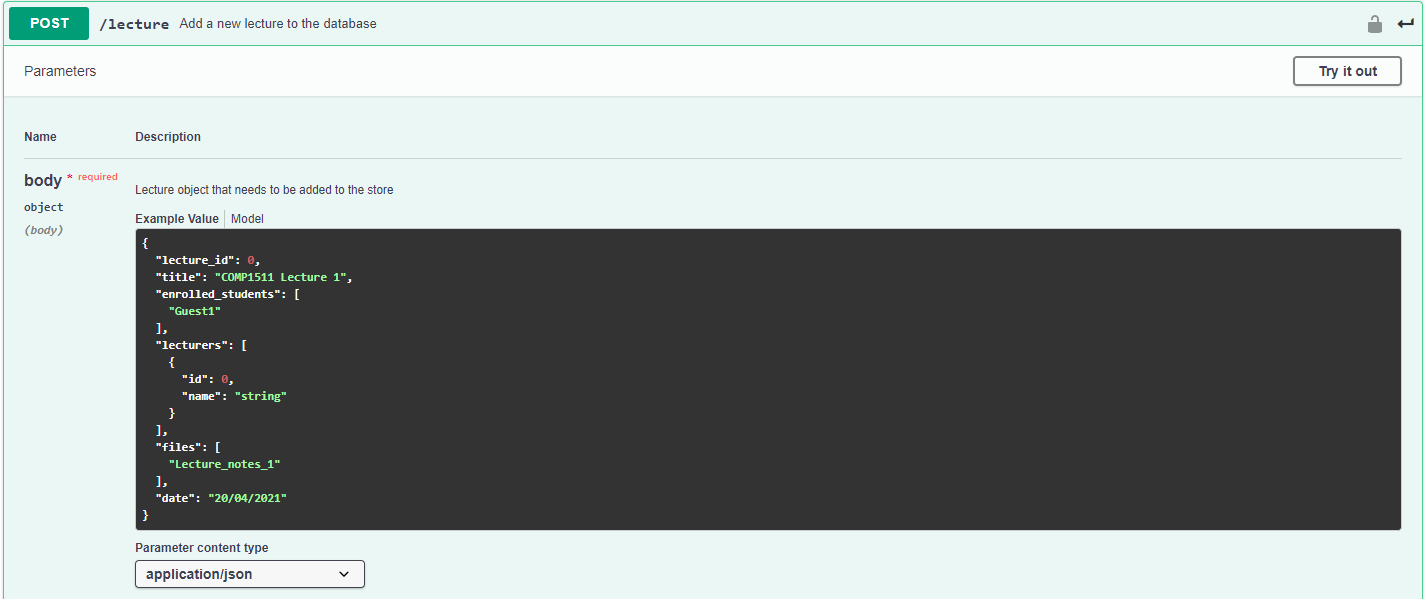
\includegraphics[scale=0.6]{backend_post_sample}
  \caption{Lecture POST Request}
\end{figure}

\newpage
\subsection{Requirements}
The requirements listed below will be in the general form as specific API calls for each 
component have not been completely finalised. Moreover, the requirements for the backend 
component will be adjusted and changed in accordance with the needs of the other components. 

\subsection{Functional Requirements}

\textbf{API}
    \begin{enumerate}
    \item Users can retrieve data
    \item Users can change data
    \item Users can delete data
    \item Users can create data
    \end{enumerate}

\textbf{Database}
    \begin{enumerate}
    \item Admins can view database entries
    \item Admins can edit database entries
    \item Admins can create database entries
    \item Admins can delete database entries
    \end{enumerate}

\subsection{Non-Functional Requirements}
  \begin{enumerate}
    \item Usability - The feature must be efficient and effective
    \item Performance - The feature must process queries within a reasonable timeframe
    \item Learnabilty - The feature must be easy to learn and use
    \end{enumerate}

\subsection{Evaluating Results}
The evaluation criterion which will be used to determine the success of the backend components in satisfying its purpose and requirements.

\begin{enumerate}
    \item Performance: Does the feature process queries within a reasonable timeframe
    \item Usability/Learnabilty: Whether the Feature is easy to learn and use
    \item Functional Requirements: Does the feature correctly satisify each requirement
\end{enumerate}